\let\negmedspace\undefined
\let\negthickspace\undefined
\documentclass[journal,12pt,onecolumn]{IEEEtran}
\usepackage{cite}
\usepackage{amsmath,amssymb,amsfonts,amsthm}
\usepackage{algorithmic}
\usepackage{graphicx}
\graphicspath{{./figs/}} 
\usepackage{textcomp}
\usepackage{xcolor}
\usepackage{txfonts}
\usepackage{listings}
\usepackage{enumitem}
\usepackage{mathtools}
\usepackage{gensymb}
\usepackage{comment}
\usepackage{caption}
\usepackage[breaklinks=true]{hyperref}
\usepackage{tkz-euclide} 
\usepackage{listings}
\usepackage{gvv}                                        
%\def\inputGnumericTable{}                                 
\usepackage[latin1]{inputenc}     
\usepackage{xparse}
\usepackage{color}                                            
\usepackage{array}                                            
\usepackage{longtable}                                       
\usepackage{calc}                                             
\usepackage{multirow}
\usepackage{multicol}
\usepackage{hhline}                                           
\usepackage{ifthen}                                           
\usepackage{lscape}
\usepackage{tabularx}
\usepackage{array}
\usepackage{float}
\newtheorem{theorem}{Theorem}[section]
\newtheorem{problem}{Problem}
\newtheorem{proposition}{Proposition}[section]
\newtheorem{lemma}{Lemma}[section]
\newtheorem{corollary}[theorem]{Corollary}
\newtheorem{example}{Example}[section]
\newtheorem{definition}[problem]{Definition}
\newcommand{\BEQA}{\begin{eqnarray}}
	\newcommand{\EEQA}{\end{eqnarray}}
\newcommand{\define}{\stackrel{\triangle}{=}}
\theoremstyle{remark}
\newtheorem{rem}{Remark}

\newcommand{\ihat}{\mathbf {\hat \imath}}
\newcommand{\jhat}{\mathbf {\hat \jmath}}
\newcommand{\vect}[1]{\mathbf #1}



\title{CH: CHEMICAL ENGINEERING}
\author{EE25BTECH11042 - Nipun Dasari}
\date{   }


\begin{document}
	
	\bibliographystyle{IEEEtran}
	\vspace{3cm}
	
	\maketitle
	\begin{enumerate}
		\item Is there any good show \underline{\hspace{2cm}} television tonight?
		
		\hfill{\brak{\text{GATE CH 2025}}}
		
		\begin{multicols}{4}
			\begin{enumerate}
				\item in
				\item at
				\item within
				\item on
			\end{enumerate}
		\end{multicols}
		
		\item As the police officer was found guilty of embezzlement, he was \underline{\hspace{2cm}} dismissed from the service in accordance with the Service Rules.
		
		\hfill{\brak{\text{GATE CH 2025}}}
		
		\begin{multicols}{2}
			\begin{enumerate}
				\item sumptuously
				\item brazenly
				\item unintentionally
				\item summarily
			\end{enumerate}
		\end{multicols}
		
		\item The sum of the following infinite series is:
		\[
		\frac{1}{1!} + \frac{1}{2!} + \frac{1}{3!} + \frac{1}{4!} + \frac{1}{5!} + \cdot\cdot\cdot
		\]
		
		\hfill{\brak{\text{GATE CH 2025}}}
		
		\begin{multicols}{2}
			\begin{enumerate}
				\item $1+e$
				\item $e-1$
				\item $e$
				\item $1$
			\end{enumerate}
		\end{multicols}
		
		\item A thin wire is used to construct all the edges of a cube of $1$ m side by bending, cutting and soldering the wire. If the wire is $12$ m long, what is the minimum number of cuts required to construct the wire frame to form the cube?
		
		\hfill{\brak{\text{GATE CH 2025}}}
		
		\begin{multicols}{2}
			\begin{enumerate}
				\item $3$
				\item $4$
				\item $1$
				\item $12$
			\end{enumerate}
		\end{multicols}
		
		\item The figures I, II and III are parts of a sequence. Which one of the following options comes next in the sequence at IV?
		\begin{figure}[h]
			\centering
			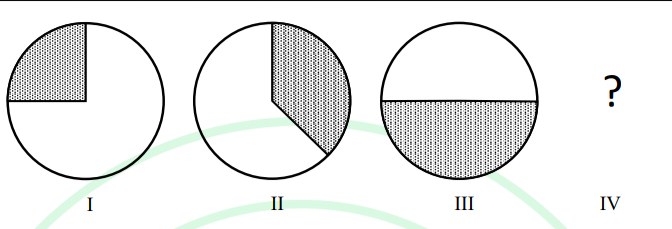
\includegraphics[width=0.8\columnwidth]{q5.png}
			\caption*{}
			\label{fig:q5}
		\end{figure}
		
		\hfill{\brak{\text{GATE CH 2025}}}
		
		\begin{figure}[h]
			\centering
			\begin{multicols}{2}
				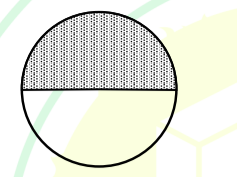
\includegraphics[width=0.4\columnwidth]{q5A.png}\par
				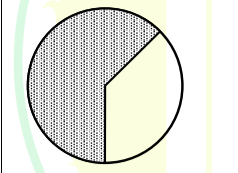
\includegraphics[width=0.4\columnwidth]{q5B.png}\par
			\end{multicols}
			\begin{multicols}{2}
				
\includegraphics[width=0.4\columnwidth]{q5C.png}\par
				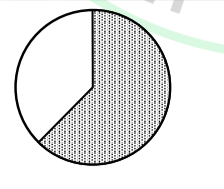
\includegraphics[width=0.4\columnwidth]{q5D.png}\par
			\end{multicols}
			\caption*{}
			\label{fig:q5_options}
		\end{figure}
		
		\item "Why do they pull down and do away with crooked streets, I wonder, which are my delight, and hurt no man living? Every day the wealthier nations are pulling down one or another in their capitals and their great towns: they do not know why they do it; neither do I. It ought to be enough, surely, to drive the great broad ways which commerce needs and which are the life-channels of a modern city, without destroying all history and all the humanity in between: the islands of the past." \brak{\text{From Hilaire Belloc's "The Crooked Streets"}}
		
		Based only on the information provided in the above passage, which one of the following statements is true?
		
		\hfill{\brak{\text{GATE CH 2025}}}
		
		\begin{enumerate}
			\item The author of the passage takes delight in wondering.
			\item The wealthier nations are pulling down the crooked streets in their capitals.
			\item In the past, crooked streets were only built on islands.
			\item Great broad ways are needed to protect commerce and history.
		\end{enumerate}
		
		\item Rohit goes to a restaurant for lunch at about 1 PM. When he enters the restaurant, he notices that the hour and minute hands on the wall clock are exactly coinciding. After about an hour, when he leaves the restaurant, he notices that the clock hands are again exactly coinciding. How much time \brak{\text{in minutes}} did Rohit spend at the restaurant?
		
		\hfill{\brak{\text{GATE CH 2025}}}
		
		\begin{multicols}{2}
			\begin{enumerate}
				\item $64\frac{6}{11}$
				\item $66\frac{5}{13}$
				\item $65\frac{5}{11}$
				\item $66\frac{6}{13}$
			\end{enumerate}
		\end{multicols}
		
		\item A color model is shown in the figure with color codes: Yellow \brak{Y}, Magenta \brak{M}, Cyan \brak{Cy}, Red \brak{R}, Blue \brak{Bl}, Green \brak{G}, and Black \brak{K}.
		
		\begin{figure}[h]
			\centering
			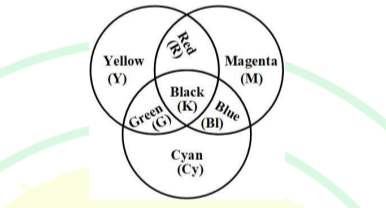
\includegraphics[width=0.4\columnwidth]{q8.png}
			\caption*{}
			\label{fig:q8}
		\end{figure}
		Which one of the following options displays the color codes that are consistent with the color model?
		
		\hfill{\brak{\text{GATE CH 2025}}}
		
		\begin{enumerate}
			\item 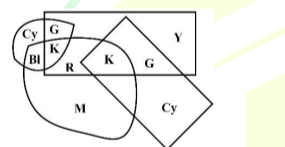
\includegraphics[width=0.7\columnwidth]{q8A.png}
			\item 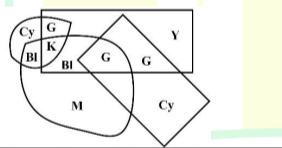
\includegraphics[width=0.7\columnwidth]{q8B.png}
			\item 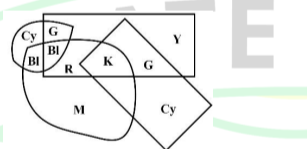
\includegraphics[width=0.7\columnwidth]{q8C.png}
			\item 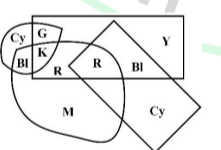
\includegraphics[width=0.7\columnwidth]{q8D.png}
		\end{enumerate}
		
		\item A circle with center at $\brak{x,y}=\brak{0.5,0}$ and radius $=0.5$ intersects with another circle with center at $\brak{x,y}=\brak{1,1}$ and radius $=1$ at two points. One of the points of intersection $\brak{x, y}$ is:
		
		\hfill{\brak{\text{GATE CH 2025}}}
		
		\begin{multicols}{2}
			\begin{enumerate}
				\item $\brak{0,0}$
				\item $\brak{0.2, 0.4}$
				\item $\brak{0.5, 0.5}$
				\item $\brak{1,2}$
			\end{enumerate}
		\end{multicols}
		
		\item An object is said to have an n-fold rotational symmetry if the object, rotated by an angle of $\frac{2\pi}{n}$ is identical to the original. Which one of the following objects exhibits 4-fold rotational symmetry about an axis perpendicular to the plane of the screen? Note: The figures shown are representative.
		
		\hfill{\brak{\text{GATE CH 2025}}}
		
		\begin{figure}[h]
			\centering
			\begin{multicols}{2}
				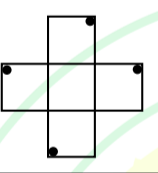
\includegraphics[width=0.3\columnwidth]{q10A.png}\par
				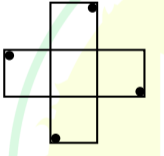
\includegraphics[width=0.3\columnwidth]{q10B.png}\par
			\end{multicols}
			\begin{multicols}{2}
				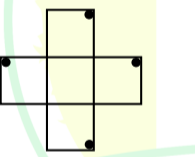
\includegraphics[width=0.3\columnwidth]{q10C.png}\par
				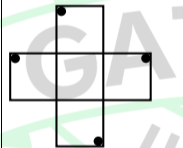
\includegraphics[width=0.3\columnwidth]{q10D.png}\par
			\end{multicols}
			\caption*{}
			\label{fig:q10_options}
		\end{figure}
		
		\item To manufacture paper from \brak{i} \underline{\hspace{2cm}}, \brak{ii} \underline{\hspace{2cm}} must be freed from the binding matrix of \brak{iii} \underline{\hspace{2cm}} in the pulping step. Which one of the following is the CORRECT option to fill in the gaps \brak{i}, \brak{ii} and \brak{iii}?
		
		\hfill{\brak{\text{GATE CH 2025}}}
		
		\begin{enumerate}
			\item \brak{i} wood, \brak{ii} cellulose fibers, \brak{iii} lignin
			\item \brak{i} lignin, \brak{ii} cellulose fibers, \brak{iii} wood
			\item \brak{i} lignin, \brak{ii} wood, \brak{iii} cellulose fibers
			\item \brak{i} wood, \brak{ii} lignin, \brak{iii} cellulose fibers
		\end{enumerate}
		
		\item Consider a Cartesian coordinate system defined over a 3-dimensional vector space with orthogonal unit basis vectors $\hat{i}$, $\hat{j}$ and $\hat{k}$. Let vector $a=\sqrt{2}\hat{i}+\frac{1}{\sqrt{2}}\hat{j}+\hat{k},$ and vector $b=\frac{1}{\sqrt{2}}\hat{i}+\sqrt{2}\hat{j}-\hat{k}.$ The inner product of these vectors $\brak{a\cdot b}$ is
		
		\hfill{\brak{\text{GATE CH 2025}}}
		
		\begin{multicols}{2}
			\begin{enumerate}
				\item $0$
				\item $1$
				\item $-1$
				\item $2$
			\end{enumerate}
		\end{multicols}
		
		\item Consider two complex numbers $z_{1}=1-i$ and $z_{2}=i$. The argument of $z_{1}z_{2}$ is
		
		\hfill{\brak{\text{GATE CH 2025}}}
		
		\begin{multicols}{4}
			\begin{enumerate}
				\item $0$
				\item $\frac{\pi}{4}$
				\item $\frac{\pi}{2}$
				\item $\pi$
			\end{enumerate}
		\end{multicols}
		
		\item A box contains 3 identical green balls and 7 identical blue balls. Two balls are randomly drawn without replacement from the box. The probability of drawing 1 green and 1 blue ball is
		
		\hfill{\brak{\text{GATE CH 2025}}}
		
		\begin{enumerate}
			\item $\frac{{}^{3}P_{1}\times{}^{7}P_{1}}{{}^{10}P_{2}}$
			\item $\frac{{}^{10}P_{3}\times{}^{10}P_{7}}{{}^{10}P_{2}}$
			\item $\frac{{}^{10}C_{3}\times{}^{10}C_{7}}{{}^{10}C_{2}}$
			\item $\frac{{}^{3}C_{1}\times{}^{7}C_{1}}{{}^{10}C_{2}}$
		\end{enumerate}
		
		\item The number of independent intensive variables that need to be specified to determine the thermodynamic state of a ternary mixture at vapor-liquid-liquid equilibrium is
		
		\hfill{\brak{\text{GATE CH 2025}}}
		
		\begin{multicols}{4}
			\begin{enumerate}
				\item 0
				\item 1
				\item 2
				\item 3
			\end{enumerate}
		\end{multicols}
		
		\item The boundary of a system does not allow exchange of either mass or energy \brak{\text{in the form of heat and/or work}} with the surroundings. The system is termed
		
		\hfill{\brak{\text{GATE CH 2025}}}
		
		\begin{multicols}{2}
			\begin{enumerate}
				\item Isolated
				\item Open
				\item Adiabatic
				\item Closed
			\end{enumerate}
		\end{multicols}
		
		\item In industrial heat exchanger design, the overall heat transfer coefficient $U$ is estimated from the equation
		\[ \frac{1}{U} = \frac{1}{h_i} + \frac{1}{h_o} \]
		where $h_i$ and $h_o$ are the convective heat transfer coefficients on the inner and outer side of the tube, respectively. This is valid for \brak{i} \underline{\hspace{2cm}} tube of \brak{ii} \underline{\hspace{2cm}} thermal conductivity.
		Which one of the following is the CORRECT option to fill in the gaps \brak{i} and \brak{ii}?
		
		\hfill{\brak{\text{GATE CH 2025}}}
		
		\begin{enumerate}
			\item \brak{i} thick-walled, \brak{ii} high
			\item \brak{i} thin-walled, \brak{ii} high
			\item \brak{i} thin-walled, \brak{ii} low
			\item \brak{i} thick-walled, \brak{ii} low
		\end{enumerate}
		
		\item The sum of the components of the force due to pressure and shear at the solid-fluid boundary of a solid body in the direction normal to the flow is
		
		\hfill{\brak{\text{GATE CH 2025}}}
		
		\begin{multicols}{2}
			\begin{enumerate}
				\item Drag
				\item Friction
				\item Lift
				\item Buoyancy
			\end{enumerate}
		\end{multicols}
		
		\item Choose the CORRECT option for pathlines, streaklines and streamlines for a STEADY flow field.
		
		\hfill{\brak{\text{GATE CH 2025}}}
		
		\begin{enumerate}
			\item All three lines are identical
			\item Only pathlines and streaklines are identical
			\item Only pathlines and streamlines are identical
			\item Only streamlines and streaklines are identical
		\end{enumerate}
		
		\item Choose the CORRECT ordering of the diameter $d$ of the different types of pores in a solid catalyst.
		
		\hfill{\brak{\text{GATE CH 2025}}}
		
		\begin{enumerate}
			\item $d_{\text{Micro-pore}} < d_{\text{Macro-pore}} < d_{\text{Meso-pore}}$
			\item $d_{\text{Macro-pore}} < d_{\text{Meso-pore}} < d_{\text{Micro-pore}}$
			\item $d_{\text{Meso-pore}} < d_{\text{Micro-pore}} < d_{\text{Macro-pore}}$
			\item $d_{\text{Micro-pore}} < d_{\text{Meso-pore}} < d_{\text{Macro-pore}}$
		\end{enumerate}
		
		\item Schmidt number is defined as
		
		\hfill{\brak{\text{GATE CH 2025}}}
		
		\begin{multicols}{2}
			\begin{enumerate}
				\item $\frac{\text{Mass Diffusivity}}{\text{Thermal Diffusivity}}$
				\item $\frac{\text{Momentum Diffusivity}}{\text{Mass Diffusivity}}$
				\item $\frac{\text{Momentum Diffusivity}}{\text{Thermal Diffusivity}}$
				\item $\frac{\text{Thermal Diffusivity}}{\text{Mass Diffusivity}}$
			\end{enumerate}
		\end{multicols}
		
		\item If $k$ is the mass transfer coefficient and $D_v$ is the molecular diffusivity, which one of the following statements is NOT CORRECT with respect to mass transfer theories?
		
		\hfill{\brak{\text{GATE CH 2025}}}
		
		\begin{enumerate}
			\item For Film theory, $k \propto D_v$
			\item For Penetration theory, $k \propto D_v^{1/3}$
			\item For Surface Renewal theory, $k \propto D_v^{1/2}$
			\item For Boundary Layer theory, $k \propto D_v^{2/3}$
		\end{enumerate}
		
		\item Choose the CORRECT statement that describes the dependence of the variance $\brak{\sigma_{\Theta}^2}$ of the residence time distribution \brak{RTD} with respect to the number of tanks \brak{n} in the Tanks-in-Series model of non-ideal reactors.
		
		\hfill{\brak{\text{GATE CH 2025}}}
		
		\begin{enumerate}
			\item $\sigma_{\Theta}^2$ monotonically increases with $n$
			\item $\sigma_{\Theta}^2$ first increases and then decreases with $n$
			\item $\sigma_{\Theta}^2$ first decreases and then increases with $n$
			\item $\sigma_{\Theta}^2$ monotonically decreases with $n$
		\end{enumerate}
		
		\item The vortex shedding meter is primarily used for measuring
		
		\hfill{\brak{\text{GATE CH 2025}}}
		
		\begin{multicols}{2}
			\begin{enumerate}
				\item Fluid Flow Rate
				\item Liquid Level
				\item Fluid Temperature
				\item Fluid Pressure
			\end{enumerate}
		\end{multicols}
		
		\item Choose the transfer function that best fits the output response to a unit step input change shown in the figure
		\begin{figure}[h]
			\centering
			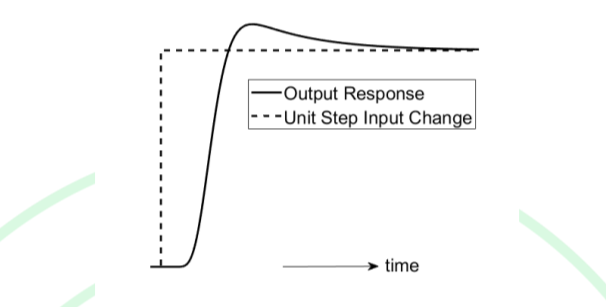
\includegraphics[width=0.5\columnwidth]{q25.png}
			\caption*{}
			\label{fig:q25}
		\end{figure}
		
		\hfill{\brak{\text{GATE CH 2025}}}
		
		\begin{enumerate}
			\item $\frac{\brak{\alpha s + 1}e^{-\theta s}}{\brak{\tau_1 s + 1}\brak{\tau_2 s + 1}^2}$
			\item $\frac{\brak{\alpha s + 1}e^{-\theta s}}{\brak{\tau_1 s + 1}\brak{\tau_2 s + 1}}$
			\item $\frac{\brak{\alpha s + 1}}{\brak{\tau_1 s + 1}\brak{\tau_2 s + 1}^2}$
			\item $\frac{\brak{\alpha s + 1}^2e^{-\theta s}}{\brak{\tau_1 s + 1}\brak{\tau_2 s + 1}^2}$
		\end{enumerate}
		
		\item The capital cost $\brak{C_C}$ of an industrial equipment varies with its capacity $\brak{S}$ as $C_C \propto S^{\beta}$. The rule-of-thumb value of the exponent $\beta$ is
		
		\hfill{\brak{\text{GATE CH 2025}}}
		
		\begin{multicols}{4}
			\begin{enumerate}
				\item $0.4$
				\item $0.6$
				\item $0.8$
				\item $1.0$
			\end{enumerate}
		\end{multicols}
		
		\item In the production of polyvinyl chloride \brak{PVC} from ethylene and chlorine, the sequential order of reactions is
		
		\hfill{\brak{\text{GATE CH 2025}}}
		
		\begin{multicols}{2}
			\begin{enumerate}
				\item Chlorination followed by Dehydrochlorination
				\item Dehydrochlorination followed by Chlorination
				\item Hydrogenation followed by Chlorination
				\item Dehydrochlorination followed by Hydrogenation
			\end{enumerate}
		\end{multicols}
		
		\item In the CONTACT PROCESS for manufacturing sulphuric acid, the reaction converting SO$_2$ to SO$_3$ is
		
		\hfill{\brak{\text{GATE CH 2025}}}
		
		\begin{multicols}{2}
			\begin{enumerate}
				\item Exothermic and reversible
				\item Endothermic and reversible
				\item Exothermic and irreversible
				\item Endothermic and irreversible
			\end{enumerate}
		\end{multicols}
		
		\item Choose the option that correctly matches the items in Group 1 with those in Group 2.
		\begin{table}[h]
			\centering
			\begin{tabular}{ll}
				\hline
				\textbf{Group 1} & \textbf{Group 2} \\
				\hline
				\brak{P} Coking & \brak{I} Prolonged exposure of catalyst to high temperature \\
				\brak{Q} Poisoning & \brak{II} Deposition of carbonaceous material on catalyst surface \\
				\brak{R} Sintering & \brak{III} Irreversible chemisorption of molecules on active sites of catalyst \\
				\hline
			\end{tabular}
			\caption*{}
			\label{tab:q29}
		\end{table}
		
		\hfill{\brak{\text{GATE CH 2025}}}
		
		\begin{enumerate}
			\item \brak{P} - \brak{III}, \brak{Q} - \brak{I}, \brak{R} -\brak{II}
			\item \brak{P} -\brak{II}, \brak{Q} - \brak{III}, \brak{R}-\brak{I}
			\item \brak{P} - \brak{II}, \brak{Q} - \brak{I}, \brak{R} - \brak{III}
			\item \brak{P} - \brak{I}, \brak{Q} - \brak{III}, \brak{R} - \brak{II}
		\end{enumerate}
		
		\item Which of the following statements regarding multiple effect evaporators is/are TRUE?
		
		\hfill{\brak{\text{GATE CH 2025}}}
		
		\begin{enumerate}
			\item The pressure of the effect with fresh steam is the lowest for both forward feed and backward feed.
			\item Backward feed is preferred over forward feed for cold feed.
			\item Backward feed is preferred over forward feed for highly viscous concentrated product.
			\item The temperature of the effect with fresh steam is the lowest for both forward feed and backward feed.
		\end{enumerate}
		
		\item Consider an enzymatic reaction that follows Michaelis-Menten kinetics. Let $K_M$, $S$, and $V_{max}$ denote the Michaelis constant, substrate concentration, and maximum reaction rate, respectively. Which of the following statements is/are TRUE?
		
		\hfill{\brak{\text{GATE CH 2025}}}
		
		\begin{enumerate}
			\item For $S \ll K_M$, the reaction is apparent first-order in $S$.
			\item For $S \gg K_M$, the reaction rate is nearly independent of $S$.
			\item For $S = K_M$, the rate of reaction equals $V_{max}$.
			\item $K_M$ is independent of the total enzyme concentration.
		\end{enumerate}
		
		\item The following data is given for a ternary $ABC$ gas mixture at $12$ MPa and $308$ K:
		\begin{table}[h]
			\centering
			\begin{tabular}{llll}
				Component $i \to$ & $A$ & $B$ & $C$ \\
				\hline
				$y_i$ & $0.55$ & $0.20$ & $0.25$ \\
				$\hat{\phi}_i$ & $0.75$ & $0.80$ & $0.95$ \\
			\end{tabular}
			\caption*{}
			\label{tab:q32}
		\end{table}
		$y_i$: mole fraction of component $i$ in the gas mixture \\
		$\hat{\phi}_i$: fugacity coefficient of component $i$ in the gas mixture at $12$ MPa and $308$ K \\
		The fugacity of the gas mixture is \underline{\hspace{2cm}} MPa \brak{\text{rounded off to 3 decimal place}}
		
		\hfill{\brak{\text{GATE CH 2025}}}
		
		\item Ideal nonreacting gases $A$ and $B$ are contained inside a perfectly insulated chamber, separated by a thin partition, as shown in the figure. The partition is removed, and the two gases mix till final equilibrium is reached. The change in total entropy for the process is \underline{\hspace{2cm}} J/K \brak{\text{rounded off to 1 decimal place}}. \\
		GIVEN: Universal gas constant $R = 8.314$ J/\brak{mol K}
		\begin{figure}[h]
			\centering
			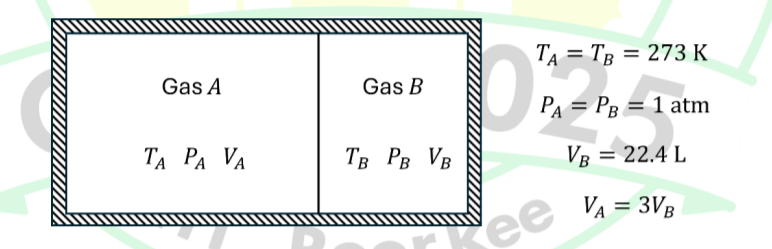
\includegraphics[width=0.6\columnwidth]{q33.png}
			\caption*{}
			\label{fig:q33}
		\end{figure}
		
		\hfill{\brak{\text{GATE CH 2025}}}
		
		\item Oil is extracted from mustard seeds having $20$ wt\% oil and $80$ wt\% solids, using hexane as a solvent. After extraction, the hexane-free residual cake contains $1$ wt\% oil. Assuming negligible dissolution of cake in hexane, the percentage oil recovery in hexane is \underline{\hspace{2cm}}\% \brak{\text{rounded off to the nearest integer}}.
		
		\hfill{\brak{\text{GATE CH 2025}}}
		
		\item The residence-time distribution \brak{RTD} function of a reactor \brak{\text{in} min^{-1}} is
		 \begin{align}
		 E\brak{t} = \begin{cases} 1 - 2t, & t \le 0.5 \text{ min} \\ 0, & t > 0.5 \text{ min} \end{cases} 
		 \end{align}
		The mean residence time of the reactor is \underline{\hspace{2cm}} min \brak{\text{rounded off to 2 decimal places}}.
		
		\hfill{\brak{\text{GATE CH 2025}}}
		
		\item Consider a Cartesian coordinate system with orthogonal unit basis vectors $\hat{i}, \hat{j}$ defined over a domain: $x, y \in [0,1]$. Choose the condition for which the divergence of the vector field $\mathbf{v} = ax\hat{i} - by\hat{j}$ is zero.
		
		\hfill{\brak{\text{GATE CH 2025}}}
		
		\begin{enumerate}
			\item $a - b = 0$
			\item $a < b$
			\item $a > b$
			\item $a + b = 0$
		\end{enumerate}
		
		\item A probability distribution function is given as
		\[ p\brak{x} = \begin{cases} 1/a, & x \in \brak{0, a} \\ 0, & \text{otherwise} \end{cases} \]
		where $a$ is a positive constant. For a function $f\brak{x} = x^2$, the expectation of $f\brak{x}$ is
		
		\hfill{\brak{\text{GATE CH 2025}}}
		
		\begin{multicols}{2}
			\begin{enumerate}
				\item $\frac{a^2}{3}$
				\item $\frac{a^3}{3}$
				\item $\frac{2a^2}{3}$
				\item $\frac{2a^3}{3}$
			\end{enumerate}
		\end{multicols}
		
		\item A hot plate is placed in contact with a cold plate of a different thermal conductivity as shown in the figure. The initial temperature \brak{\text{at time t = 0}} of the hot plate and cold plate are $T_h$ and $T_c$, respectively. Assume perfect contact between the plates.\\
		\begin{figure}[h]
			\centering
			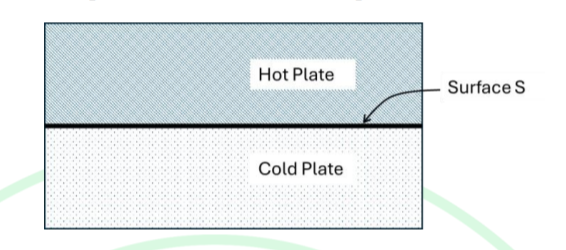
\includegraphics[width=0.6\columnwidth]{q38.png}
			\caption*{}
			\label{fig:q38}
		\end{figure} \\

		Which one of the following is an appropriate boundary condition at the surface S for solving the unsteady state, one-dimensional heat conduction equations for the hot plate and cold plate for $t > 0$?

	\newpage	
		\hfill{\brak{\text{GATE CH 2025}}}
		
		\begin{enumerate}
			\item Temperature at S is same for both the plates
			\item Gradient of temperature at S is same for both the plates
			\item Gradient of temperature vanishes at S
			\item Temperature at S is the average of $T_h$ and $T_c$
		\end{enumerate}
		
		\item The first-order irreversible liquid phase reaction $A \longrightarrow B$ occurs inside a constant volume \brak{V} isothermal CSTR with the initial steady state conditions shown in the figure. The gain, in $\frac{\text{kmol/m}^3}{\text{m}^3\text{/h}}$, of the transfer function relating the reactor effluent $A$ concentration, $c_A$, to the inlet flow rate, $F$, is
		
		\begin{figure}[h]
			\centering
			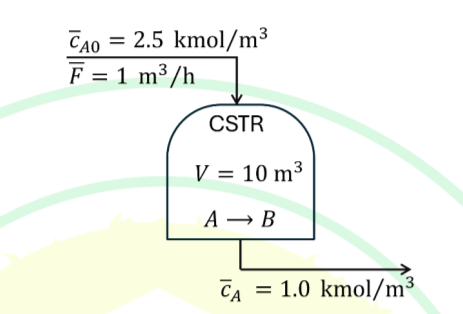
\includegraphics[width=0.6\columnwidth]{q39.png}
			\caption*{}
			\label{fig:q39}
		\end{figure}
		
		\hfill{\brak{\text{GATE CH 2025}}}
		
		\begin{multicols}{4}
			\begin{enumerate}
				\item $1.2$
				\item $0.4$
				\item $0.6$
				\item $0.8$
			\end{enumerate}
		\end{multicols}
		
		\item $500$ mg of a dry adsorbent is added to a beaker containing $100$ mL solution of concentration $100$ mg phenol/\brak{\text{L solution}}. The adsorbent is separated out after $5$ h of rigorous mixing. If the residual concentration in the solution after separating the adsorbent is $30$ mg phenol/\brak{\text{L solution}}, the amount of phenol adsorbed \brak{\text{in mg per gram of dry adsorbent}} is
		
		\hfill{\brak{\text{GATE CH 2025}}}
		
		\begin{multicols}{4}
			\begin{enumerate}
				\item $7$
				\item $14$
				\item $28$
				\item $18$
			\end{enumerate}
		\end{multicols}
		
		\item A catalyst particle is modeled as a symmetrical double cone solid as shown in the figure. For each conical sub-part, the radius of the base is $r$ and the height is $h$. The sphericity of the particle is given by
				\begin{figure}[h]
			\centering
			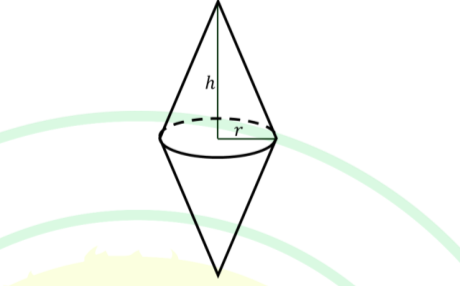
\includegraphics[width=0.6\columnwidth]{q41.png}
			\caption*{}
			\label{fig:q41}
		\end{figure}
		
		\hfill{\brak{\text{GATE CH 2025}}}
		
		\begin{enumerate}
			\item $\frac{2 \brak{r^2h^2}^{1/3}}{r\sqrt{r^2 + h^2}}$
			\item $\frac{\brak{r^2h^2}^{1/3}}{r\sqrt{r^2 + h^2}}$
			\item $\frac{2 \brak{r^2h^2}^{2/3}}{r\sqrt{r^2 + h^2}}$
			\item $\frac{\brak{r^2h^2}^{2/3}}{r\sqrt{r^2 + h^2}}$
		\end{enumerate}
		
		\item A zero-order gas phase reaction $A \rightarrow B$ with rate $\brak{-r_A} = k = 100$ mol/\brak{\text{L min}} is carried out in a mixed flow reactor of volume $1$ L. Pure $A$ is fed to the reactor at a rate of $1$ mol/min. At time $t = 0$, the outlet flow is stopped while the inlet flow rate and reactor temperature remain unchanged. Assume that the reactor was operating under steady state before the flow was stopped \brak{t < 0}. The rate of consumption of $A$, $-dC_A/dt$, in mol/\brak{\text{L min}}, at $t = 1$ min is
		
		\hfill{\brak{\text{GATE CH 2025}}}
		
		\begin{multicols}{4}
			\begin{enumerate}
				\item $63.2$
				\item $36.8$
				\item $90.6$
				\item $99.0$
			\end{enumerate}
		\end{multicols}
		
		\item For a steady state, fully developed laminar flow of a Newtonian fluid through a cylindrical pipe at a constant volumetric flow rate, which of the following statements regarding the pressure drop across the pipe \brak{\Delta P} is/are TRUE?
		
		\hfill{\brak{\text{GATE CH 2025}}}
		
		\begin{enumerate}
			\item $\Delta P$ increases with fluid viscosity
			\item $\Delta P$ increases with pipe length
			\item $\Delta P$ increases with pipe diameter
			\item $\Delta P$ remains unchanged with fluid viscosity
		\end{enumerate}
		
		\item Consider the differential equation
		\[ \frac{dy}{dx} + \frac{y}{x} = 0 \]
		Choose the CORRECT option\brak{s} for the solution $y$.
		
		\hfill{\brak{\text{GATE CH 2025}}}
		
		\begin{enumerate}
			\item $y = x + c$ ; $c$ is a constant
			\item $y = \frac{c}{x}$; $c$ is a constant
			\item $y = -x + c$ ; $c$ is a constant
			\item $y = 0$
		\end{enumerate}
		
		\item Consider the matrix
		\begin{align}
		\vec{A} = \myvec{2 & 3 \\ 1 & 2} 
	    \end{align}
		The eigenvalues of the matrix are $0.27$ and \underline{\hspace{2cm}} \brak{\text{rounded off to 2 decimal places}}.
		
		\hfill{\brak{\text{GATE CH 2025}}}
		
		\item The Newton-Raphson method is used to find the root of
		\[ f\brak{x} \equiv x^2 - x - 1 = 0 \]
		Starting with an initial guess $x^{\brak{0}} = 1$, the second iterate $x^{\brak{2}}$ is \underline{\hspace{2cm}} \brak{\text{rounded off to 2 decimal places}}.
		
		\hfill{\brak{\text{GATE CH 2025}}}
		
		\item Consider moist air with absolute humidity of $0.02$ \brak{\text{kg moisture}}/\brak{\text{kg dry air}}at $1$ bar pressure. The vapour pressure of water is given by the equation
		\[ \ln P^{sat} = 12 - \frac{4000}{T - 40} \]
		where $P^{sat}$ is in bar and $T$ is in K. The molecular weight of water and dry air are $18$ kg/kmol and $29$ kg/kmol, respectively. The dew temperature of the moist air is \underline{\hspace{2cm}} $\degree$C \brak{\text{rounded off to the nearest integer}}.
		
		\hfill{\brak{\text{GATE CH 2025}}}
		
		\item An ideal monoatomic gas is contained inside a cylinder-piston assembly connected to a Hookean spring as shown in the figure. The piston is frictionless and massless. The spring constant is $10$ kN/m. At the initial equilibrium state \brak{shown in the figure}, the spring is unstretched. The gas is expanded reversibly by adding $362.5$ J of heat. At the final equilibrium state, the piston presses against the stoppers. Neglecting the heat loss to the surroundings, the final equilibrium temperature of the gas is \underline{\hspace{2cm}} K \brak{\text{rounded off to the nearest integer}}. \\
		GIVEN: For a monoatomic ideal gas, $C_v = \frac{3}{2}R$, where $R = 8.314$ J/\brak{mol K}
		\begin{figure}[h]
			\centering
			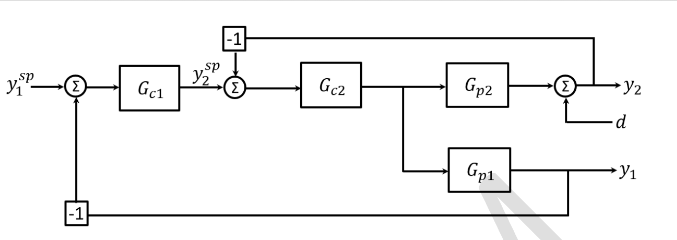
\includegraphics[width=0.7\columnwidth]{q48.png}
			\caption*{}
			\label{fig:q48}
		\end{figure}
		
		\hfill{\brak{\text{GATE CH 2025}}}
		
		\item A leaf filter is operated at $1$ atm \brak{gauge}. The volume of filtrate collected \brak{\text{V in} m^3} is related with the volumetric flow rate of the filtrate \brak{\text{q in m$^3$/s}} as:
		\[ \frac{1}{q} = \frac{1}{dV/dt} = 50 V + 100 \]
		The volumetric flow rate of the filtrate at $1$ hour is \underline{\hspace{2cm}} $\times 10^{-3}$ m$^3$/s \brak{\text{rounded off to 2 decimal places}}.
		
		\hfill{\brak{\text{GATE CH 2025}}}
		
		\item An adiabatic pump of efficiency $40\%$ is used to increase the water pressure from $200$ kPa to $600$ kPa. The flow rate of water is $600$ L/min. The specific heat of water is $4.2$ kJ/\brak{kg \degree C}. Assuming water is incompressible with a density of $1000$ kg/m$^3$, the maximum temperature rise of water across the pump is \underline{\hspace{2cm}}$\degree$C \brak{\text{rounded off to 3 decimal places}}.
		
		\hfill{\brak{\text{GATE CH 2025}}}
		
		\item Water flowing at $70$ kg/min is heated from $25$ $\degree$C to $65$ $\degree$C in a counter-flow double pipe heat exchanger using hot oil. The oil enters at $110$ $\degree$C and exits at $65$ $\degree$C. If the overall heat transfer coefficient is $300$ W/\brak{m^2 K}, the heat exchanger area is \underline{\hspace{2cm}} m$^2$ \brak{\text{rounded off to 1 decimal place}}. \\
		GIVEN: Specific heat of water and oil are $4.2$ kJ/\brak{kg \degree C} and $2$ kJ/\brak{kg \degree C}, respectively.
		
		\hfill{\brak{\text{GATE CH 2025}}}
		
		\item Consider laminar flow of water over a wide flat plate maintained at a uniform temperature of $50 \degree$C as shown in the figure. The freestream velocity and temperature of water are $1.0$ m/s \brak{parallel to the plate} and $20 \degree$C, respectively. The distance $x$ from the leading edge, at which the thermal boundary layer thickness $\delta_T = 0.01$ m, is \underline{\hspace{2cm}} m \brak{\text{rounded off to 1 decimal place}}. \\
		GIVEN: kinematic viscosity: $\nu = 1.0 \times 10^{-6}$ m$^2$/s \\
		Prandtl number: $Pr = 7.01$ \\
		velocity boundary layer thickness: $\delta_H = \frac{4.91x}{\sqrt{Vx/\nu}}$
		\begin{figure}[h]
			\centering
			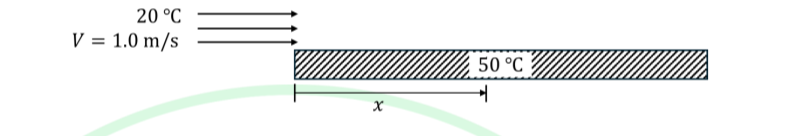
\includegraphics[width=0.8\columnwidth]{q52.png}
			\caption*{}
			\label{fig:q52}
		\end{figure}
		
		\hfill{\brak{\text{GATE CH 2025}}}
		
		\item An electrical wire of $2$ mm diameter and $5$ m length is insulated with a plastic layer of thickness $2$ mm and thermal conductivity $k = 0.1$ W/\brak{m K}. It is exposed to ambient air at $30 \degree$C. For a current of $5$ A, the potential drop across the wire is $2$ V. The air-side heat transfer coefficient is $20$ W/\brak{m^2 K}. Neglecting the thermal resistance of the wire, the steady state temperature at the wire-insulation interface is \underline{\hspace{2cm}}$\degree$C \brak{\text{rounded off to 1 decimal place}}.
		
		\hfill{\brak{\text{GATE CH 2025}}}
		
		\item A binary $AB$ liquid mixture containing $30$ mol\% $A$ is subjected to differential \brak{Rayleigh} distillation at atmospheric pressure in order to recover $60$ mol\% $A$ in the distillate. Assuming a constant relative volatility $\alpha_{AB} = 2.2$, the average composition of the collected distillate is \underline{\hspace{2cm}} mol\% $A$ \brak{\text{rounded off to nearest integer}}.
		
		\hfill{\brak{\text{GATE CH 2025}}}
		
		\item Gas containing $0.8$ mol\% component $A$ is to be scrubbed with pure water in a packed bed column to reduce the concentration of $A$ to $0.1$ mol\% in the exit gas. The inlet gas and water flow rates are $0.1$ kmol/s and $3.0$ kmol/s, respectively. For the dilute system, both the operating and equilibrium curves are considered linear. If the slope of the equilibrium line is $24$, the number of transfer units, based on the gas side, $N_{OG}$ is \underline{\hspace{2cm}} \brak{\text{rounded off to 1 decimal place}}.
		
		\hfill{\brak{\text{GATE CH 2025}}}
		
		\item Solute A is absorbed from a gas into water in a packed bed operating at steady state. The absorber operating pressure and temperature are $1$ atm and $300$ K, respectively. At the gas-liquid interface $y_i = 1.5 x_i$ where $y_i$ and $x_i$ are the interfacial gas and liquid mole fractions of A, respectively. At a particular location in the absorber, the mole fractions of A in the bulk gas and in the bulk water are $0.02$ and $0.002$, respectively. If the ratio of the local individual mass transfer coefficients for the transport of A on the gas-side \brak{k_y} to that on the water-side \brak{k_x}, $\frac{k_y}{k_x} = 2$, then $y_i$ equals \underline{\hspace{2cm}} \brak{\text{rounded off to 3 decimal place}}
		
		\hfill{\brak{\text{GATE CH 2025}}}
		
		\item Components $A$ and $B$ form an azeotrope. The saturation vapour pressures of $A$ and $B$ at the boiling temperature of the azeotrope are $87$ kPa and $72.7$ kPa, respectively. The azeotrope composition is \underline{\hspace{2cm}} mol\% $A$ \brak{\text{rounded off to the nearest integer}}. \\
		GIVEN:
		\[ \ln\frac{\gamma_A}{\gamma_B} = 0.9\brak{x_B^2 - x_A^2} \]
		where $x_i$ and $\gamma_i$ are the liquid phase mole fraction and activity coefficient of component $i$, respectively.
		
		\hfill{\brak{\text{GATE CH 2025}}}
		
		\item The reaction $A \rightarrow \text{products}$ with reaction rate, $\brak{-r_A} = kC_A^3$, occurs in an isothermal PFR operating at steady state. The conversion \brak{X} at two axial locations \brak{1 and 2} of the PFR is shown in the figure. The value of $l_1/l_2$ is \underline{\hspace{2cm}} \brak{\text{rounded off to 2 decimal places}}.
		\begin{figure}[h]
			\centering
			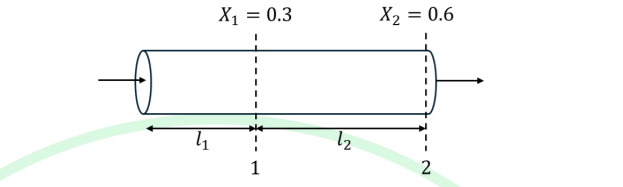
\includegraphics[width=0.6\columnwidth]{q58.png}
			\caption*{}
			\label{fig:q58}
		\end{figure}
		
		\hfill{\brak{\text{GATE CH 2025}}}
		
		\item The catalytic gas phase reaction $A \rightarrow \text{products}$ is carried out in an isothermal batch reactor of $10$ L volume using $0.1$ kg of a solid catalyst. The reaction is first-order with
		\[ \brak{-r'_A} = k'a\brak{t}C_A \]
		where $k' = 1 \frac{\text{L}}{\brak{\text{kg catalyst}}\brak{\text{h}}}$ and $C_A$ is the concentration of $A$ in mol/L. The catalyst activity $a\brak{t}$ undergoes first-order decay with rate constant $k_d = 0.01$ per hour and $a\brak{0} = 1$. The reactant conversion after $1$ day of operation is \underline{\hspace{2cm}} \brak{\text{rounded off to 2 decimal places}}.
		
		\hfill{\brak{\text{GATE CH 2025}}}
		
		\item Consider a process with transfer function
	$ G_p = \frac{2e^{-s}}{\brak{5s + 1}^2} $
		A first-order plus dead time \brak{FOPDT} model is to be fitted to the unit step process reaction curve \brak{PRC} by applying the maximum slope method. Let $\tau_m$ and $\theta_m$ denote the time constant and dead time, respectively, of the fitted FOPDT model. The value of $\tau_m / \theta_m$ is \underline{\hspace{2cm}} \brak{\text{rounded off to 2 decimal places}}. \\
		GIVEN: For $G = \frac{1}{\brak{\tau s + 1}^2}$
		the unit step output response: $y\brak{t} = 1 - \brak{1 + \frac{t}{\tau}}e^{-t/\tau}$ \\
		$\frac{dy\brak{t}}{dt} = \frac{t}{\tau^2}e^{-t/\tau}$ \\
		$\frac{d^2y\brak{t}}{dt^2} = \frac{1}{\tau^2}\brak{1 - \frac{t}{\tau}}e^{-t/\tau}$
		
		\hfill{\brak{\text{GATE CH 2025}}}
		
		\item Methanol is produced by the reversible, gas-phase hydrogenation of carbon monoxide as
		\[ CO + 2H_2 \rightleftharpoons CH_3OH \]
		$CO$ and $H_2$ are charged to a reactor and the reaction proceeds to equilibrium at $453$ K and $2$ atm. The reaction equilibrium constant, which depends only on the temperature, is $1.68$ at the reaction conditions. The mole fraction of $H_2$ in the product is $0.4$. Assuming ideal gas behaviour, the mole fraction of methanol in the product is \underline{\hspace{2cm}} \brak{\text{rounded off to 2 decimal places}}.
		
		\hfill{\brak{\text{GATE CH 2025}}}
		
		\item The block diagram of a series cascade control system \brak{\text{with time in minutes}} is shown in the figure. For $\tau_I = 8$ min and $K_{cs} = 1$, the maximum value of $K_{cm}$, below which the cascade control system is stable, is \underline{\hspace{2cm}} \brak{\text{rounded off to the nearest integer}}.
		\begin{figure}[h]
			\centering
			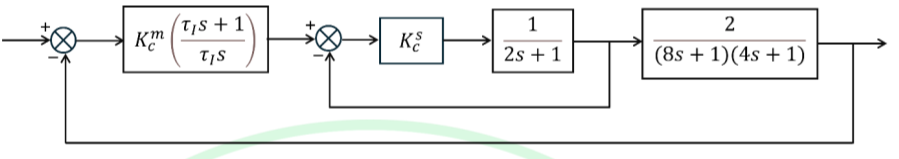
\includegraphics[width=0.6\columnwidth]{q62.png}
			\caption*{}
			\label{fig:q62}
		\end{figure}
		\hfill{\brak{\text{GATE CH 2025}}}
		
		\item It is proposed to install thermal insulation in a residence to save on the summer-monsoon season air-conditioning costs. The estimated yearly saving is $20$ thousand rupees. The cost of installation of the insulation is $150$ thousand rupees. The life of the insulation is $12$ years. For a compound interest rate of $9\%$ per annum, the minimum salvage value of the insulation for which the proposal is competitive, is \underline{\hspace{2cm}} thousand rupees \brak{\text{rounded off to nearest integer}}.
		
		\hfill{\brak{\text{GATE CH 2025}}}
		
		\item Consider the flowsheet in the figure for manufacturing $C$ via the reaction $A + B \longrightarrow C$ in an isothermal CSTR. The split in the separator is perfect so that the recycle stream is free of $C$ and the product stream is pure $C$. Let $x_i$ denote the mole fraction of species $i$ \brak{\text{i = A, B, C}} in the CSTR, which is operated in excess B with $x_B/x_A = 4$. The reaction is first-order in $A$ with the reaction rate $\brak{-r_A} = k_x x_A$, where $k_x = 5.0$ kmol/\brak{m^3 h}. The reactor volume $V$ in m$^3$ is to be optimized to minimize the cost objective $J = V + 0.25R$, where $R$ is the recycle rate in kmol/h. For a product rate $P = 100$ kmol/h, the optimum value of $V$ is \underline{\hspace{2cm}} m$^3$ \brak{\text{rounded off to the nearest integer}}. \\
		GIVEN: $\frac{d}{dz}\brak{\frac{z}{1-z}} = \frac{1}{\brak{1-z}^2}$
		\begin{figure}[h]
			\centering
			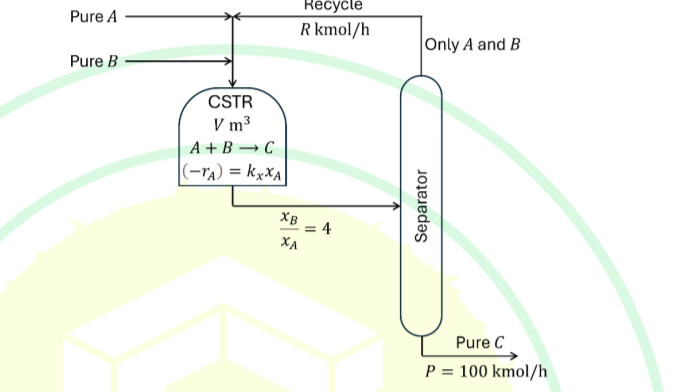
\includegraphics[width=0.6\columnwidth]{q64.png}
			\caption*{}
			\label{fig:q64}
		\end{figure}
		
		\hfill{\brak{\text{GATE CH 2025}}}
		
		\item A wet solid of $100$ kg containing $30$ wt\% moisture is to be dried to $2$ wt\% moisture in a tray dryer. The critical moisture content is $10$ wt\% and the equilibrium moisture content is $1$ wt\%. The drying rate during the constant rate period is $10$ kg/\brak{h m^2}. The drying curve in the falling rate period is linear. If the drying area is $5$ m$^2$, the time required for drying is \underline{\hspace{2cm}} h \brak{\text{rounded off to 1 decimal place}}. \\
		Note: All the moisture values given are on dry-solid basis.
		
		\hfill{\brak{\text{GATE CH 2025}}}
	\end{enumerate}
	
\end{document}